% Options for packages loaded elsewhere
\PassOptionsToPackage{unicode}{hyperref}
\PassOptionsToPackage{hyphens}{url}
\PassOptionsToPackage{dvipsnames,svgnames,x11names}{xcolor}
%
\documentclass[
  letterpaper,
  DIV=11,
  numbers=noendperiod,
  oneside]{scrartcl}

\usepackage{amsmath,amssymb}
\usepackage{iftex}
\ifPDFTeX
  \usepackage[T1]{fontenc}
  \usepackage[utf8]{inputenc}
  \usepackage{textcomp} % provide euro and other symbols
\else % if luatex or xetex
  \usepackage{unicode-math}
  \defaultfontfeatures{Scale=MatchLowercase}
  \defaultfontfeatures[\rmfamily]{Ligatures=TeX,Scale=1}
\fi
\usepackage{lmodern}
\ifPDFTeX\else  
    % xetex/luatex font selection
\fi
% Use upquote if available, for straight quotes in verbatim environments
\IfFileExists{upquote.sty}{\usepackage{upquote}}{}
\IfFileExists{microtype.sty}{% use microtype if available
  \usepackage[]{microtype}
  \UseMicrotypeSet[protrusion]{basicmath} % disable protrusion for tt fonts
}{}
\makeatletter
\@ifundefined{KOMAClassName}{% if non-KOMA class
  \IfFileExists{parskip.sty}{%
    \usepackage{parskip}
  }{% else
    \setlength{\parindent}{0pt}
    \setlength{\parskip}{6pt plus 2pt minus 1pt}}
}{% if KOMA class
  \KOMAoptions{parskip=half}}
\makeatother
\usepackage{xcolor}
\usepackage[top=1in,left=1in,right=1in]{geometry}
\setlength{\emergencystretch}{3em} % prevent overfull lines
\setcounter{secnumdepth}{-\maxdimen} % remove section numbering
% Make \paragraph and \subparagraph free-standing
\ifx\paragraph\undefined\else
  \let\oldparagraph\paragraph
  \renewcommand{\paragraph}[1]{\oldparagraph{#1}\mbox{}}
\fi
\ifx\subparagraph\undefined\else
  \let\oldsubparagraph\subparagraph
  \renewcommand{\subparagraph}[1]{\oldsubparagraph{#1}\mbox{}}
\fi


\providecommand{\tightlist}{%
  \setlength{\itemsep}{0pt}\setlength{\parskip}{0pt}}\usepackage{longtable,booktabs,array}
\usepackage{calc} % for calculating minipage widths
% Correct order of tables after \paragraph or \subparagraph
\usepackage{etoolbox}
\makeatletter
\patchcmd\longtable{\par}{\if@noskipsec\mbox{}\fi\par}{}{}
\makeatother
% Allow footnotes in longtable head/foot
\IfFileExists{footnotehyper.sty}{\usepackage{footnotehyper}}{\usepackage{footnote}}
\makesavenoteenv{longtable}
\usepackage{graphicx}
\makeatletter
\def\maxwidth{\ifdim\Gin@nat@width>\linewidth\linewidth\else\Gin@nat@width\fi}
\def\maxheight{\ifdim\Gin@nat@height>\textheight\textheight\else\Gin@nat@height\fi}
\makeatother
% Scale images if necessary, so that they will not overflow the page
% margins by default, and it is still possible to overwrite the defaults
% using explicit options in \includegraphics[width, height, ...]{}
\setkeys{Gin}{width=\maxwidth,height=\maxheight,keepaspectratio}
% Set default figure placement to htbp
\makeatletter
\def\fps@figure{htbp}
\makeatother
% definitions for citeproc citations
\NewDocumentCommand\citeproctext{}{}
\NewDocumentCommand\citeproc{mm}{%
  \begingroup\def\citeproctext{#2}\cite{#1}\endgroup}
\makeatletter
 % allow citations to break across lines
 \let\@cite@ofmt\@firstofone
 % avoid brackets around text for \cite:
 \def\@biblabel#1{}
 \def\@cite#1#2{{#1\if@tempswa , #2\fi}}
\makeatother
\newlength{\cslhangindent}
\setlength{\cslhangindent}{1.5em}
\newlength{\csllabelwidth}
\setlength{\csllabelwidth}{3em}
\newenvironment{CSLReferences}[2] % #1 hanging-indent, #2 entry-spacing
 {\begin{list}{}{%
  \setlength{\itemindent}{0pt}
  \setlength{\leftmargin}{0pt}
  \setlength{\parsep}{0pt}
  % turn on hanging indent if param 1 is 1
  \ifodd #1
   \setlength{\leftmargin}{\cslhangindent}
   \setlength{\itemindent}{-1\cslhangindent}
  \fi
  % set entry spacing
  \setlength{\itemsep}{#2\baselineskip}}}
 {\end{list}}
\usepackage{calc}
\newcommand{\CSLBlock}[1]{\hfill\break\parbox[t]{\linewidth}{\strut\ignorespaces#1\strut}}
\newcommand{\CSLLeftMargin}[1]{\parbox[t]{\csllabelwidth}{\strut#1\strut}}
\newcommand{\CSLRightInline}[1]{\parbox[t]{\linewidth - \csllabelwidth}{\strut#1\strut}}
\newcommand{\CSLIndent}[1]{\hspace{\cslhangindent}#1}

\KOMAoption{captions}{tableheading}
\makeatletter
\@ifpackageloaded{tcolorbox}{}{\usepackage[skins,breakable]{tcolorbox}}
\@ifpackageloaded{fontawesome5}{}{\usepackage{fontawesome5}}
\definecolor{quarto-callout-color}{HTML}{909090}
\definecolor{quarto-callout-note-color}{HTML}{0758E5}
\definecolor{quarto-callout-important-color}{HTML}{CC1914}
\definecolor{quarto-callout-warning-color}{HTML}{EB9113}
\definecolor{quarto-callout-tip-color}{HTML}{00A047}
\definecolor{quarto-callout-caution-color}{HTML}{FC5300}
\definecolor{quarto-callout-color-frame}{HTML}{acacac}
\definecolor{quarto-callout-note-color-frame}{HTML}{4582ec}
\definecolor{quarto-callout-important-color-frame}{HTML}{d9534f}
\definecolor{quarto-callout-warning-color-frame}{HTML}{f0ad4e}
\definecolor{quarto-callout-tip-color-frame}{HTML}{02b875}
\definecolor{quarto-callout-caution-color-frame}{HTML}{fd7e14}
\makeatother
\makeatletter
\@ifpackageloaded{caption}{}{\usepackage{caption}}
\AtBeginDocument{%
\ifdefined\contentsname
  \renewcommand*\contentsname{Table of contents}
\else
  \newcommand\contentsname{Table of contents}
\fi
\ifdefined\listfigurename
  \renewcommand*\listfigurename{List of Figures}
\else
  \newcommand\listfigurename{List of Figures}
\fi
\ifdefined\listtablename
  \renewcommand*\listtablename{List of Tables}
\else
  \newcommand\listtablename{List of Tables}
\fi
\ifdefined\figurename
  \renewcommand*\figurename{Figure}
\else
  \newcommand\figurename{Figure}
\fi
\ifdefined\tablename
  \renewcommand*\tablename{Table}
\else
  \newcommand\tablename{Table}
\fi
}
\@ifpackageloaded{float}{}{\usepackage{float}}
\floatstyle{ruled}
\@ifundefined{c@chapter}{\newfloat{codelisting}{h}{lop}}{\newfloat{codelisting}{h}{lop}[chapter]}
\floatname{codelisting}{Listing}
\newcommand*\listoflistings{\listof{codelisting}{List of Listings}}
\makeatother
\makeatletter
\makeatother
\makeatletter
\@ifpackageloaded{caption}{}{\usepackage{caption}}
\@ifpackageloaded{subcaption}{}{\usepackage{subcaption}}
\makeatother
\makeatletter
\@ifpackageloaded{sidenotes}{}{\usepackage{sidenotes}}
\@ifpackageloaded{marginnote}{}{\usepackage{marginnote}}
\makeatother
\ifLuaTeX
  \usepackage{selnolig}  % disable illegal ligatures
\fi
\usepackage{bookmark}

\IfFileExists{xurl.sty}{\usepackage{xurl}}{} % add URL line breaks if available
\urlstyle{same} % disable monospaced font for URLs
\hypersetup{
  pdftitle={ORD Service Area Boundary Model Documentation},
  colorlinks=true,
  linkcolor={blue},
  filecolor={Maroon},
  citecolor={Blue},
  urlcolor={Blue},
  pdfcreator={LaTeX via pandoc}}

\title{ORD Service Area Boundary Model Documentation}
\author{}
\date{}

\begin{document}
\maketitle

\renewcommand*\contentsname{Table of contents}
{
\hypersetup{linkcolor=}
\setcounter{tocdepth}{2}
\tableofcontents
}
\begin{tcolorbox}[enhanced jigsaw, bottomtitle=1mm, colbacktitle=quarto-callout-important-color!10!white, toptitle=1mm, leftrule=.75mm, breakable, colback=white, coltitle=black, bottomrule=.15mm, arc=.35mm, left=2mm, opacityback=0, opacitybacktitle=0.6, titlerule=0mm, rightrule=.15mm, colframe=quarto-callout-important-color-frame, title=\textcolor{quarto-callout-important-color}{\faExclamation}\hspace{0.5em}{Disclaimer}, toprule=.15mm]

This document is distributed solely for the purpose of pre-dissemination
peer review under applicable information quality guidelines. It has not
been formally disseminated by the U.S. Environmental Protection Agency.
It does not represent and should not be construed to represent any
agency determination or policy.

\end{tcolorbox}

\textbf{Version 1.0}

\textbf{SDWIS Data Vintage:} 2023 (Quarter 4)

The Office of Research and Development has released a publicly available
dataset of community water system (CWS) service area boundaries (SAB).
CWS are defined as systems that provide water for human consumption
through pipes or other constructed conveyances to at least 15 service
connections or serves an average of at least 25 people year-round
{[}1{]}. Under the safe drinking water act (SDWA) and various drinking
water rules (see EPA Drinking Water Regulations) public water systems
must test and report on the quality of their drinking water. These
boundaries enable linking SDWA violations to their associated geographic
areas, and concomitantly linking treated community water system water to
their respective customers. This service area boundary dataset is a
combination of publicly available service area boundaries and modeled
boundaries. This document describes how the data was collected and
modeled and details the modeling techniques used to generate this
dataset.

\section{Summary}\label{summary}

Public water systems regulated under SDWA are required to treat their
drinking water. A sample of 931 public wells found that ``one or more
chemical contaminants were detected at concentrations greater than MCLs
or HBSLs in more than one in five (22 percent)'' of the sampled wells
(Toccalino, Norman, and Hitt 2010). This substantiates the need for
federal requirements; these samples were collected prior to treatment
and treatment processes, or dilution can substantially reduce the risk
of contaminants getting to the consumer. While federal standards help
reduce the likelihood of contaminated drinking water, of the 50,000
public water system in the US, 2,741 were in continuous health-based
violation of National Primary Drinking Water Violations in 2021 (U.S.
EPA 2022). Community water systems have testing and reporting
requirements that may increase based on the size of the system,
compliance history and local or state specific requirements. While the
source of water for a home may by a primary determinate of its quality,
the type of system, whether private, mobile home park, small community
water system, or large community water system can play an equally
important role in the ability for a system to have adequate treatment
processes. It is therefore critical that we understand where people are
sourcing their water, who is consuming the water, and how it is
delivered to their home in order to more completely understand regional
and national trends of water quality and the health impacts to the
public. This research on geographically the extent of public water use
leverages a new spatial disaggregation technique to increase the spatial
resolution of well estimates in addition to using machine learning
techniques to estimate the total number of housing units getting their
water from public sources in 2020 at the census block level. After that
is achieved we use a random forest model to associate the corresponding
public water system ID to each census block identified as ``publicly
supplied''.

The boundaries presented in this dataset are an aggregate of several
methods used to present the most accurate representation possible with
available data. These methods range in source and accuracy. Each method
is described in detail.

\subsection{SDWA Reporting Universe}\label{sdwa-reporting-universe}

The current ORD dataset (Version 1.0), uses the 2023 (Q4) release of
SDWA data. As of this release, there were a total of 49,396 active
community water systems, which primarily serve residential areas (Figure
2). There are many systems, however, which primarily wholesale water to
other systems and therefore do not have a service area boundary. The
universe of systems in our efforts is limited to currently active
community water systems which serve at least 15 service connections or
serves an average of at least 25 people for at least 60 days a year..
The total number of systems that fit this criteria for 2023 (Q4) is:
49,396

\subsection{Count of Systems by Primacy
Agency}\label{count-of-systems-by-primacy-agency}

Community water systems each fall under a primacy agency, which is
typically determined by the state which they serve. The exception to
this rule is tribal systems, which report to the EPA regional offices
directly.

\begin{figure}

\centering{

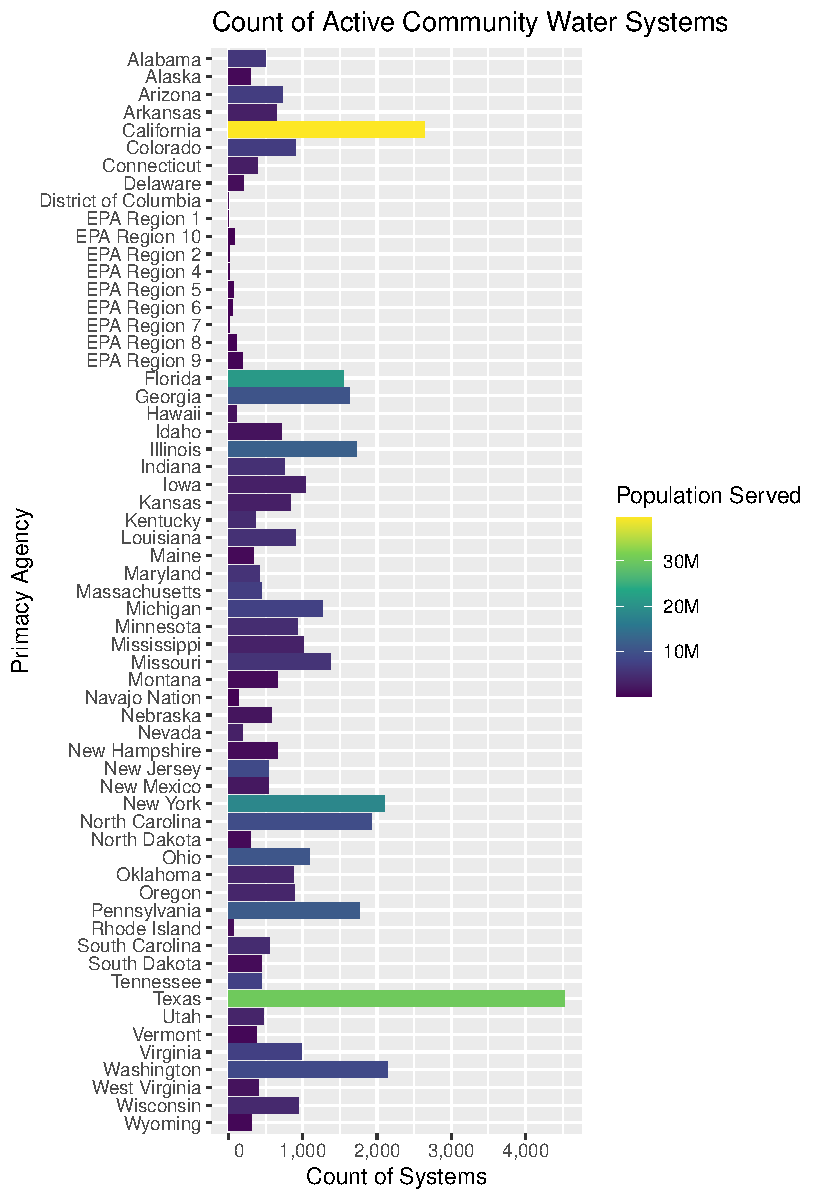
\includegraphics{Documentation_files/figure-pdf/fig-statePlot-1.pdf}

}

\caption{\label{fig-statePlot}Bar plot showing the count of active
community water systems by state, region or territory.}

\end{figure}%

\subsection{Systems by Type of Service
Area}\label{systems-by-type-of-service-area}

\begin{figure}

\centering{

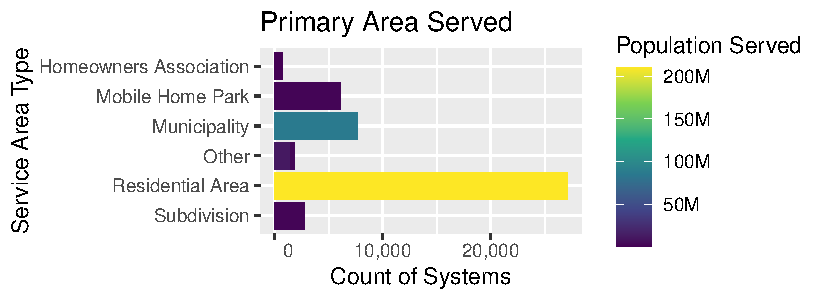
\includegraphics{Documentation_files/figure-pdf/fig-systemType-1.pdf}

}

\caption{\label{fig-systemType}Types of Active Systems in SDWA
Reporting}

\end{figure}%

\section{State Data}\label{state-data}

When detailed public water service area boundaries are publicly
available from state or municipal sources, we consider that to be the
highest quality spatial data possible. A detailed review was conducted
of available data and used to determine what would be included in the
ORD national map versus what would be modeled. Detailed descriptions of
state data are available in the state boundary appendix.

\begin{table}

\caption{\label{tbl-stateCounts}Number of system boundaries from state
and municipal sources included in the ORD dataset. The total number of
systems included is 18,374.}

\begin{minipage}{0.33\linewidth}
\begin{center}
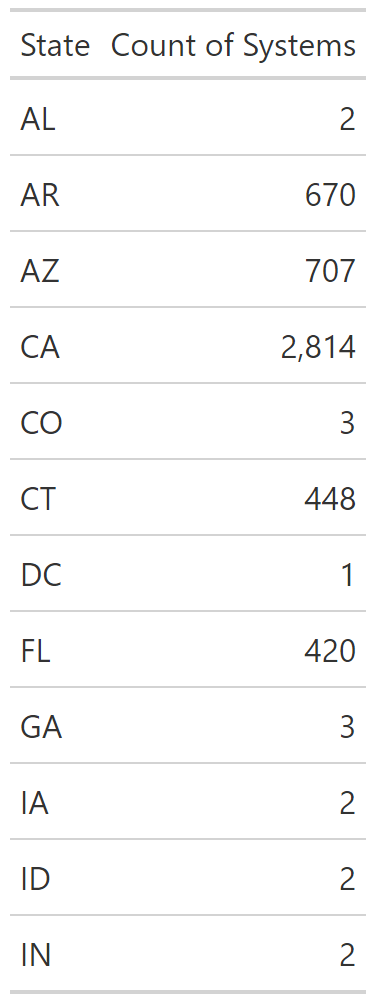
\includegraphics[width=1.25in,height=\textheight]{img/state_table_1.png}
\end{center}
\end{minipage}%
%
\begin{minipage}{0.33\linewidth}
\begin{center}
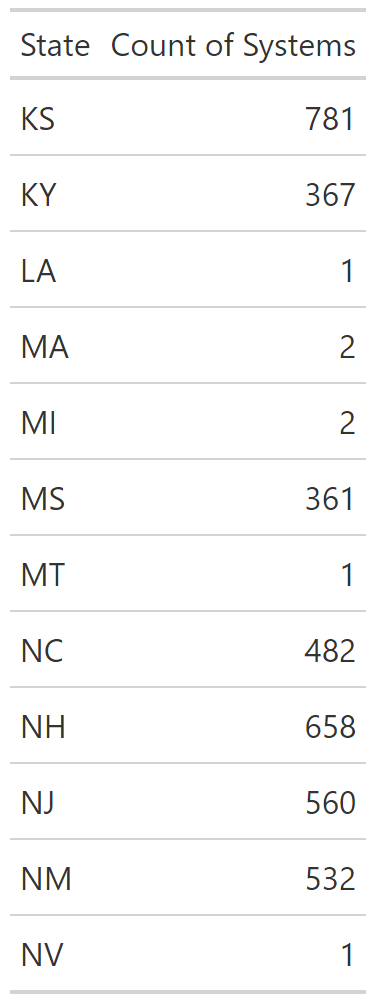
\includegraphics[width=1.25in,height=\textheight]{img/state_table_2.png}
\end{center}
\end{minipage}%
%
\begin{minipage}{0.33\linewidth}
\begin{center}
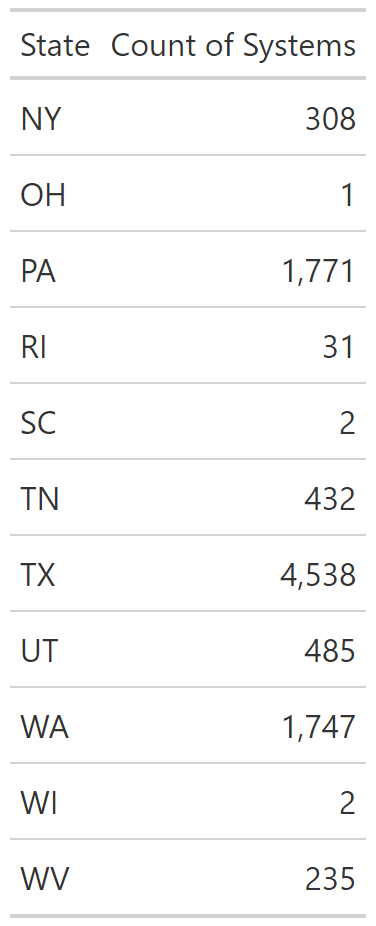
\includegraphics[width=1.25in,height=\textheight]{img/state_table_3.png}
\end{center}
\end{minipage}%

\end{table}%

\section{Place Matched Service Area
Boundaries}\label{place-matched-service-area-boundaries}

\subsection{Mobile Homes - OSM}\label{mobile-homes---osm}

Areas delineated as mobile home parks were extracted from Open Street
Map and fuzzy name matched with community water system names reported
under SDWA. To find open street map delineated areas, the point
locations for mobile home parks from Homeland Infrastructure
Foundation-Level Data (HIFLD) was intersected with areas tagged as
`residental=trailer\_park' in open street map. If a match was found, the
given names of that mobile home park (from both sources) were matched
with SDWA reported names.

\subsection{Mobile Homes - Parcels}\label{mobile-homes---parcels}

Where open street map delineated areas were not present, point locations
of mobile home parks from HIFLD were intersected with parcels from
\href{https://app.regrid.com/us\#}{REGRID}. The name of the mobile home
park was then fuzzy matched with SDWA reported system names.

\section{Modeled Service Area
Boundaries}\label{modeled-service-area-boundaries}

\subsection{Binary Water Use Model}\label{binary-water-use-model}

A decision tree model was created to determine the probability that a
census block is served by a public water system. This model was levered
in two different ways: 1.) to aid in the 1:1 matching discussed later
and 2.) as a model input (explanatory variable) for the random forest
model. The variables included are listed in Table 2. To validate the
model, public water systems from three states (New Jersey, Connecticut
\& California) were joined to census blocks to classify the intersecting
blocks as public water users. These three states were chosen based on
the completeness and detail of their service area boundaries. The final
decision tree model (Figure~\ref{fig-dt}) predicted the type of water
supply correctly in 93.14\% of blocks in the testing dataset which was
removed prior to training. The accuracy of public use (sensitivity) was
95\% and the accuracy of private use (specificity) was 81\%. A secondary
validation was performed using data from Washington, which was never
exposed to the model for training (Table~\ref{tbl-wash}) For more
details on this initial model, refer to the
\href{https://github.com/USEPA/ORD_Water_Source_2020}{2020 Water Source
Model GitHub Site}.

\begin{table}

\caption{\label{tbl-importance}Variables included in decision tree
model.}

\centering{

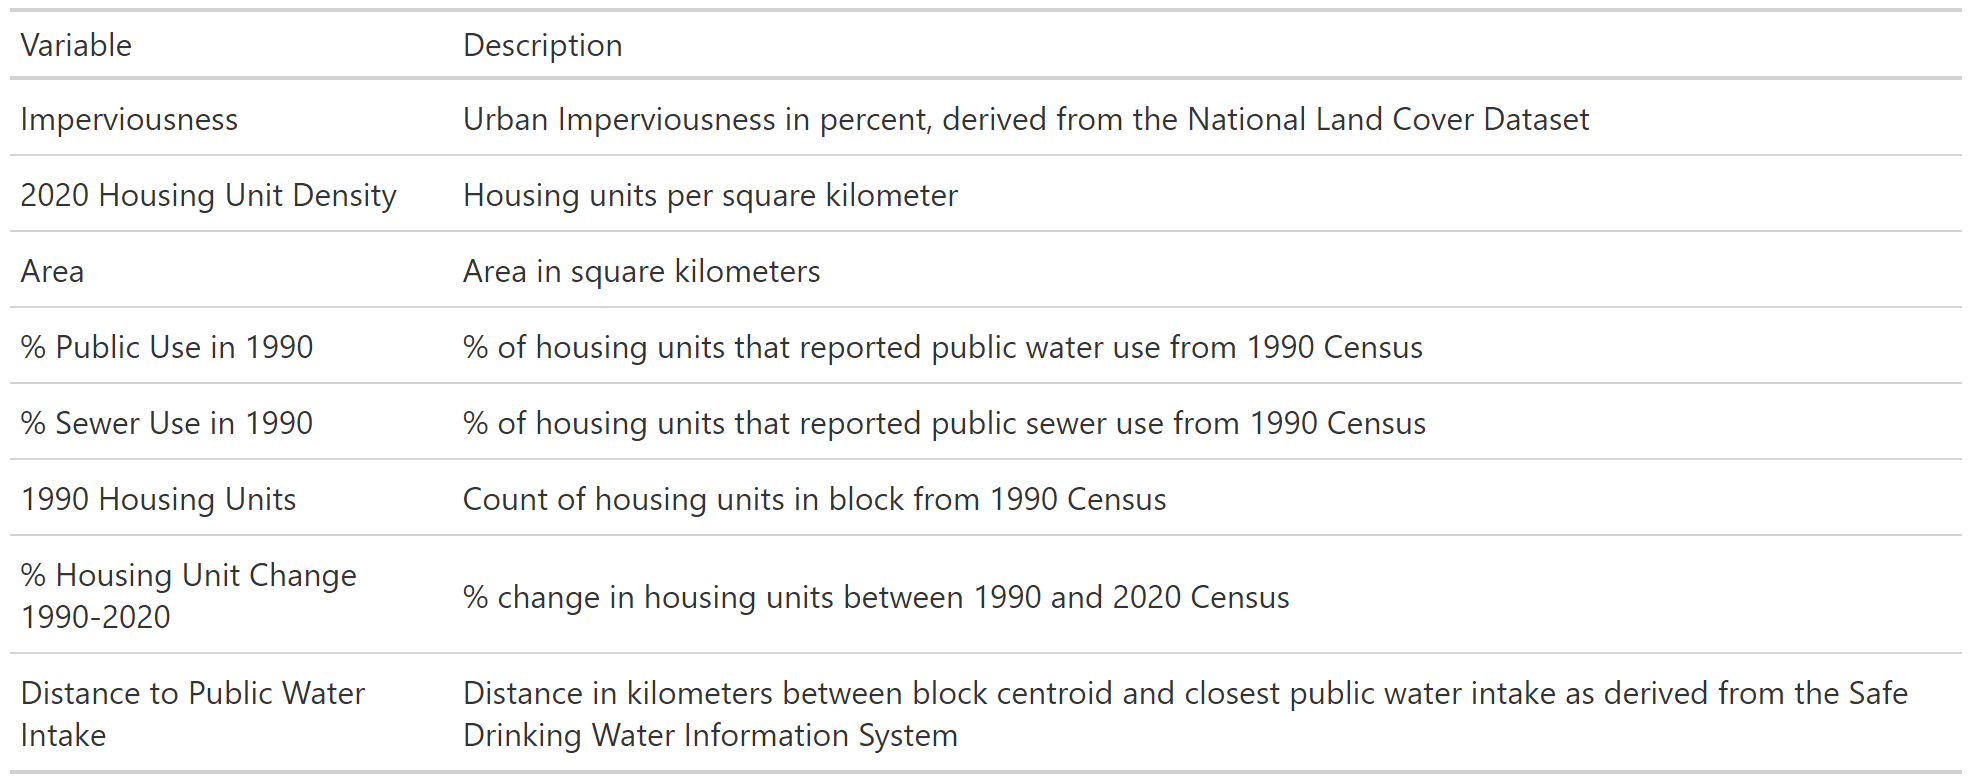
\includegraphics[width=6.57in,height=\textheight]{img/varTable.png}

}

\end{table}%

\begin{table}

\caption{\label{tbl-wash}Confusion matrix showing both decision tree
predictions for both the out of bag testing set and data from
Washington.}

\centering{

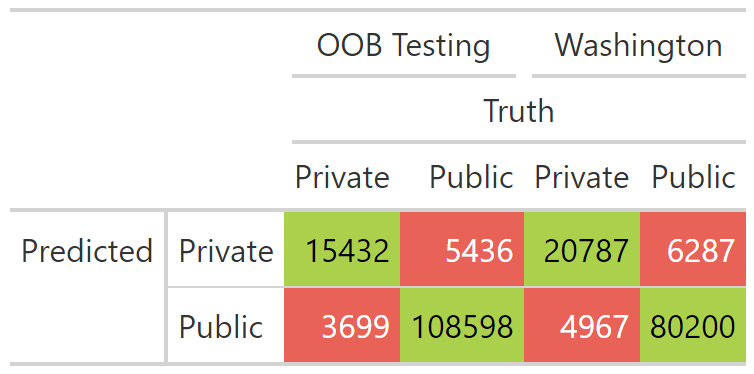
\includegraphics[width=3in,height=\textheight]{img/performance_tbl.png}

}

\end{table}%

\begin{figure}

\centering{

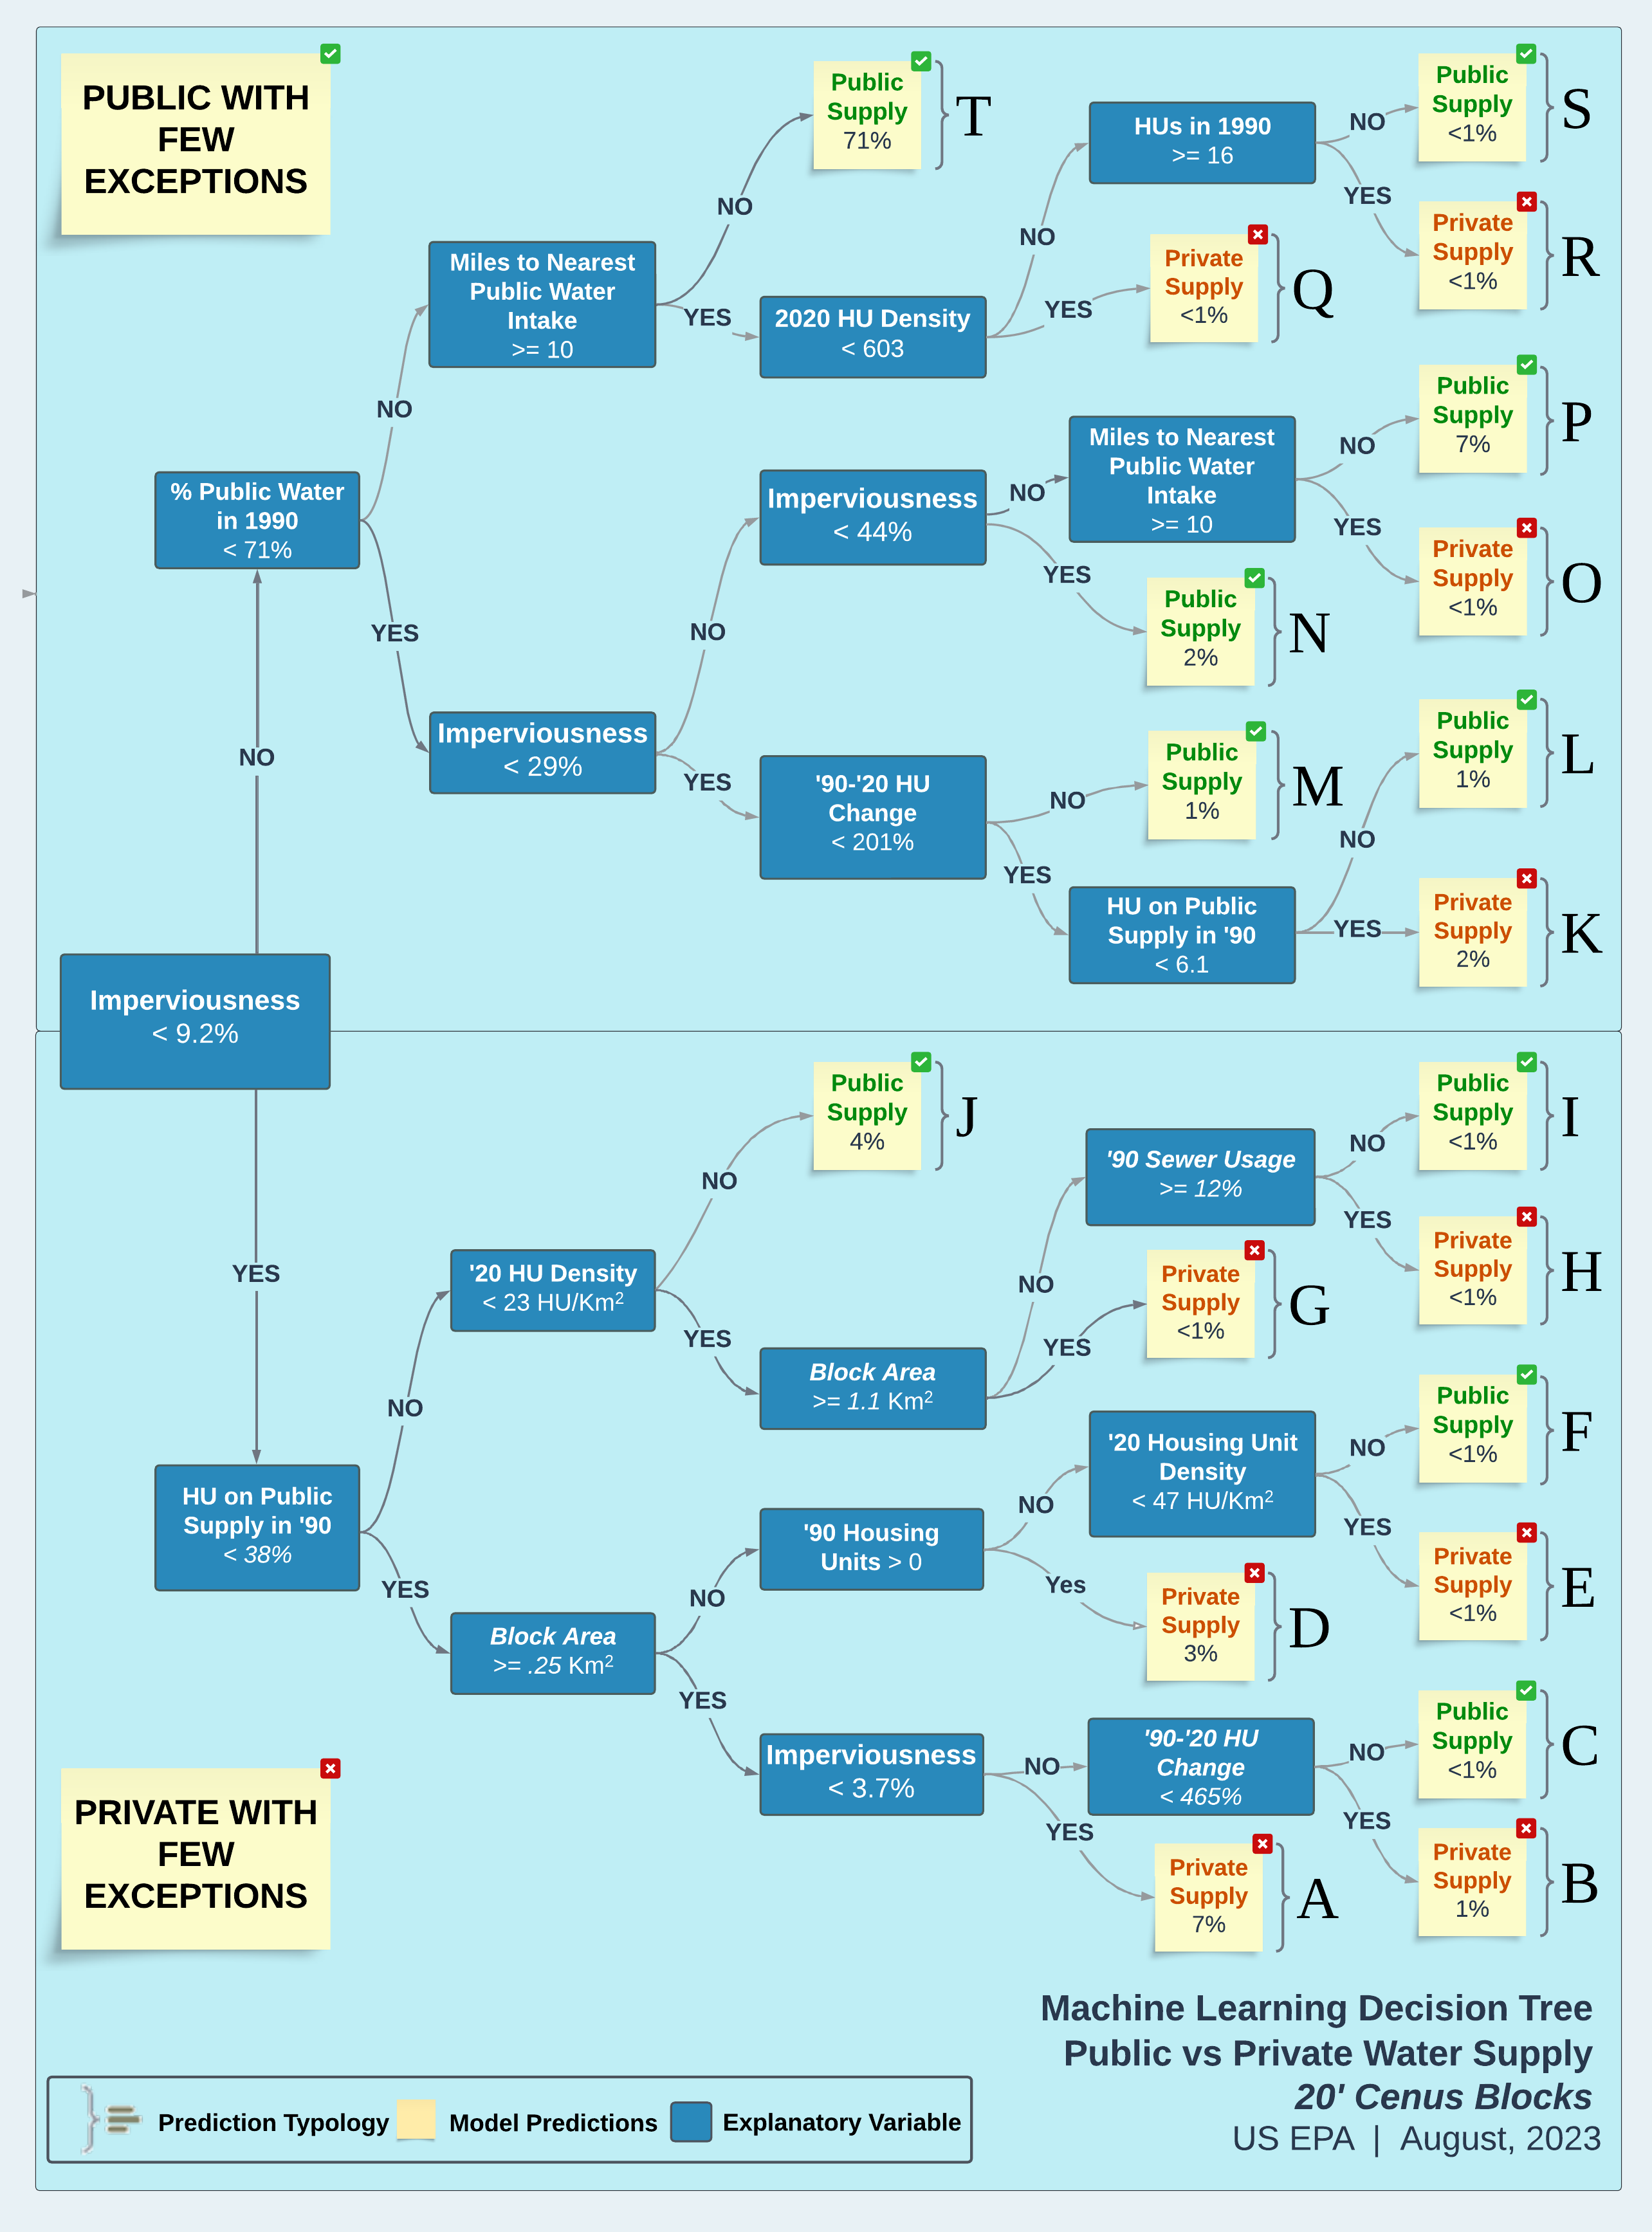
\includegraphics{img/DT.png}

}

\caption{\label{fig-dt}Visualization of decision tree to predict whether
a census block is served by a public water system.}

\end{figure}%

\subsection{1:1 Match}\label{match}

Census blocks that are predicted to be served by public water by the
binary water use model (Figure~\ref{fig-dt}) are `aggregated' or
`dissolved' spatially, meaning they are combined with any contiguous
blocks that are also estimated to be served by public water systems into
larger polygons. A public probability threshold of .7 and higher was
used to classify block as exclusively on public water. These aggregated
polygons are then spatially joined with facility locations from SDWIS,
which include intakes, wells, and treatment plants. If a single
aggregated area can only be associated with facilities from a single
public water system, that area is assigned its associated PWSID.

As a general approach to modeling, simplicity is typically preferred
over complexity. The 1:1 matching was an attempt to resolve system
assignments in a very simple way, eliminating the need for more complex
random forest modeling. Approximately 8,000 systems were assigned (or
matched) using this method. This method leveraged the decision tree
output to determine system boundary size. Since the model provided
confidence levels associated to every block, from 0=confident that that
the block is privately supplied; to 1= confident that block is publicly
supplied. We found that a value of 0.7 closely approximated the system
boundary size and shape when compared to state supplied boundaries.
After applying this criteria, we sought to match the system boundaries
to their associated PWSID. Spatially continuous blocks were aggregated
together into larger polygons.

To determine a match, we used SDWIS locations (wells, treatment plant,
intakes) and SDWA locations (reported system addresses that we geocoded)
to conduct a spatial join to the aggregated decision tree boundaries (at
0.7 confidence). The logic here is that for some systems there is only
one PWS that serves the polygon area---as opposed to a more complex
nested set of systems within a single polygon. More complex systems are
mainly associated with urban and suburban areas where the simple systems
are largely associated with smaller to mid-size towns in rural areas.
The other assumption we had was that it is more likely that a system's
infrastructure is close to the population that it serves than farther
away.

We performed a spatial join on all decision tree boundaries and SDWIS
and SDWA locations. If more than one unique system was joined, those
boundaries were returned for random forest modeling. If only one PWSID
was returned for a polygon we validated that the joins were associated
with the correct PWS. To do this we performed a graphical validation
method by regressing the service connection of the joined public water
system against the sum 2020 housing units within the modeled boundary.
Because each state uses a different formula for calculating the service
connections, these regressions had to be limited to intra-state
comparisons. In other words, the regressions coefficients could vary
widely between states, creating an ``apples-to-oranges'' comparison. The
regression was trimmed to systems that fell close to the 1-to-1
regression line. Systems that deviated from that line were removed for
later random forest matching. Figure~\ref{fig-IA} is an example of Iowa
systems that were matched using this graphical method for matching
systems.

\begin{figure}

\centering{

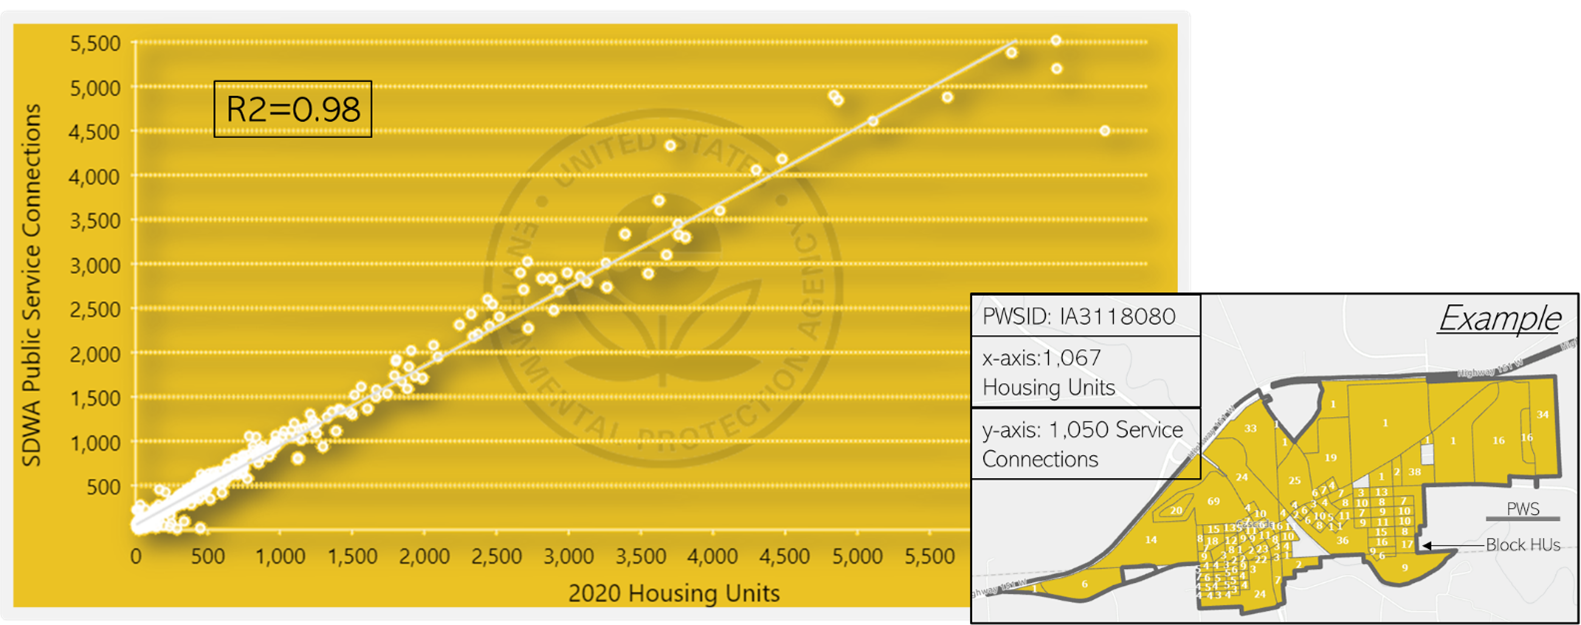
\includegraphics{img/IA_Regression.png}

}

\caption{\label{fig-IA}example of ``matched'' 1:1 systems using the
graphical regression method. These systems have a strong correlation
between housing units (x) and reported service connections (y). The
bottom right image shows how census block housing units are aggregated
per unique PWS}

\end{figure}%

\subsection{Random Forest}\label{random-forest}

The goal of the random forest model is to be able to determine what
public water system (or PWSID) a census block is most likely to be
served by. For example, a block in a rural area that is using public
water may be more likely to be close to its source water intake if it is
a very small system and more likely to be farther away if it a very
large rural water district. If you are served by a system that purchases
all of its water, the infrastructure may be farther away as well.

The random forest is set up to evaluate the relationship between a
single census block and a single point associated with a public water
system. The tabular data used to train and apply the random forest model
has one row for the relationship between every block and every unique
PWSID within 25 miles (as determined by CWS infrastructure such as
wells, treatment plants, facility addresses, and intakes). As an
example, if there are seven different facilities within twenty-five
miles of a census block, the table used for the random forest will have
seven rows for that census block. Each facility is associated with a
parent PWSID. The random forest model then predicts a probability that
the parent PWSID is serving the census block in the same row of the
table. Predictor variables can be thought of as belonging to one of two
groups:

\begin{itemize}
\tightlist
\item
  Variables that that characterize the census block
\item
  Variables that characterize the water system.
\end{itemize}

The random forest model then determines the correct interplay between
the variables to determine a probability that a particular system serves
a particular census block or is not served by a public water system at
all.

\subsubsection{Variables that Describe the Census
Block}\label{variables-that-describe-the-census-block}

\paragraph{Population}\label{population}

Variable Name: \texttt{Population}

Population is taken from the 2020 Census, obtained at the census block
level.

\paragraph{Local Population Density}\label{local-population-density}

Variable Name: \texttt{Pop\_km}

The centroid of each block is buffered by 2 miles (3,218.69 meters). The
population density is then calculated as an areal weighted population
density of census blocks that intersect the buffer. This variable
informs each block of its surroundings---in particular how dense is the
nearby city, suburb or rural area.

\paragraph{Area}\label{area}

Variable Name: \texttt{Area\_Km}

Area is calculated for each block in square kilometers using the Albers
equal area projection (crs = 5070).

\paragraph{Probability of Public
Water}\label{probability-of-public-water}

Variable Name: \texttt{Prob\_Pub}

The probability (0-1) of a block being served by public water as
estimated from the ORD water use decision tree model
(Figure~\ref{fig-dt}).

\paragraph{Buildings}\label{buildings}

Variable Name: \texttt{nBuildings}

The number of buildings within a census block that are greater then 50
square meters in area. This is calculated using microsoft building
footprints.

\paragraph{Percent Buildings}\label{percent-buildings}

Variable Name: \texttt{PctBldg}

The percent area of the census block that is covered by buildings. This
is calculated as the total area of microsoft building footprints divided
by the area of the census block.

\paragraph{Mean Building Area}\label{mean-building-area}

Variable Name: \texttt{meanBldg\_m}

The mean area in square meters of buildings within the census block.

\paragraph{Minimum Building Area}\label{minimum-building-area}

Variable Name: \texttt{minBldg\_m}

The area in square meters of the smallest building within the census
block (Only buildings greater than or equal to 50 square meters
included).

\paragraph{Maximum Building Area}\label{maximum-building-area}

Variable Name: \texttt{maxBldg\_m}

The area in square meters of the largest building within the census
block (Only buildings greater than or equal to 50 square meters
included).

\paragraph{Standard Deviation of Building
Area}\label{standard-deviation-of-building-area}

Variable Name: \texttt{sdBldg\_m}

The standard deviation of area of buildings in square meters within a
census block.

\paragraph{Rural / Urban}\label{rural-urban}

Variable Name: \texttt{PctRural}

The census defined urban / rural classifier; A binary classification, in
which to qualify as an urban area, the block identified must encompass
at least 2,000 housing units or have a population of at least 5,000 for
2020 (census block level).

\paragraph{Mean Residential Acres}\label{mean-residential-acres}

Variable Name: \texttt{meanResAcres}

The mean value in acres of parcels within the census block that are
zoned for residential use.

\paragraph{Count of Parcels}\label{count-of-parcels}

Variable Name: \texttt{nParcels}

The total count of parcels within the census block.

\paragraph{Count of Mobile Homes}\label{count-of-mobile-homes}

Variable Name: \texttt{MH\_Count}

The count of mobile home communities within a census block as derived
from the (Homeland Infrastructure Foundation Level
database){[}https://hifld-geoplatform.opendata.arcgis.com/datasets/mobile-home-parks/explore{]}.

\paragraph{Mobile Home Size}\label{mobile-home-size}

Variable Name: \texttt{MH\_Size}

The cumulative size of mobile home parks within a census block
representing the number of mobile home units. This variable is presented
as a factor.

\textbf{Possible Values:}

\begin{longtable}[]{@{}ll@{}}
\toprule\noalign{}
Value & Description \\
\midrule\noalign{}
\endhead
\bottomrule\noalign{}
\endlastfoot
`50' & \textless50 Mobile Homes \\
`75' & 50-100 Mobile Homes \\
`100' & \textgreater100 Mobile Homes \\
\end{longtable}

\subsubsection{Variables that Describe the Closest
Systems}\label{variables-that-describe-the-closest-systems}

\paragraph{Distance}\label{distance}

Variable Name: \texttt{Facility\_Dist} The distance in meters between
the census block centroid and a single point from SDWIS for a system.

\paragraph{Distance Rank}\label{distance-rank}

Variable Name: \texttt{Dist\_Rank}

Describes the closeness rank of the particular facility being measured
to. For example, if \texttt{Dist\_Rank\ =\ 5}, there would be 4 other
facility points closer to the centroid of that census block.

\paragraph{Facility Type}\label{facility-type}

Variable Name: \texttt{Facility\_Type}

The type of system point that was used in the distance calculation.
Options include:

\begin{itemize}
\tightlist
\item
  ``Well''
\item
  ``Treatment Plant''
\item
  ``Consecutive Connection''
\item
  ``Intake''
\item
  ``Other''
\end{itemize}

The `Other' Category contains less frequent data and data used when
there are no wells, intakes or treatment plants associated with a
system. Some examples of less frequent locations are springs, reservoirs
and infiltration zones. This class also contains the office addresses of
systems as reported to SDWIS which are typically within a service area
but are also known to be unreliable depending on the system. Office
locations were geolocated and curated to only include street
intersections or better.

\paragraph{Population Served}\label{population-served}

Variable Name: \texttt{Population\_Served\_Count}

The reported population that is served by the system in SDWA reporting.

\paragraph{Connections}\label{connections}

Variable Name: \texttt{Service\_Connections\_Count}

The reported number of service connections within a system in SDWA
reporting.

\paragraph{Distance to Center of
System}\label{distance-to-center-of-system}

Variable Name: \texttt{Ctr\_Dist}

If a system has more than one SDWIS point (intakes, wells treatment
plants etc\ldots) the mean center of all points is calculated and
measured in meters from the centroid of the census block. If only one
point exists within a system, this value will be identical to
\texttt{Facility\_Dist}.

\paragraph{System Type}\label{system-type}

Variable Name: \texttt{Service\_Area\_Type}

The Primary type of area that is served by the public water system.

\textbf{Possible Values:}

\begin{itemize}
\tightlist
\item
  `Homeowners Association'
\item
  `Mobile Home Park'
\item
  `Multiple'
\item
  `Municipality'\\
\item
  `Other'
\item
  `Residential Area'
\item
  `Subdivision'
\end{itemize}

\paragraph{Sub-County Match}\label{sub-county-match}

Variable Name: \texttt{SubCounty\_Match}

Reflects a classified Jaro-Winkler string distance between the census
place the census block is within and the `City Served' of the public
water system associated with the point being measured to.

\begin{longtable}[]{@{}ll@{}}
\toprule\noalign{}
Jaro-Winkler Distance & Classification \\
\midrule\noalign{}
\endhead
\bottomrule\noalign{}
\endlastfoot
\textless0.1 & ``Full Match'' \\
\textgreater0.1 \& \textless0.3 & ``Partial Match'' \\
≥0.3 & ``No Match'' \\
if no census sub county & ``No SubCounty'' \\
if no city served & ``No City Served'' \\
\end{longtable}

\paragraph{Place Match}\label{place-match}

Variable Name: \texttt{Place\_Match}

Reflects a classified Jaro-Winkler string distance between the census
place the census block is within and the `City Served' of the public
water system associated with the point being measured to.

\begin{longtable}[]{@{}ll@{}}
\toprule\noalign{}
Jaro-Winkler Distance & Classification \\
\midrule\noalign{}
\endhead
\bottomrule\noalign{}
\endlastfoot
\textless0.1 & ``Full Match'' \\
\textgreater0.1 \& \textless0.3 & ``Partial Match'' \\
≥0.3 & ``No Match'' \\
if no census place & ``No Place'' \\
if no city served & ``No City Served'' \\
\end{longtable}

\paragraph{County Match}\label{county-match}

Variable Name: \texttt{County\_Match}

A categorical value denoting whether the county that the census block is
within matches a county reported to be served by the system being
measured.

\textbf{Possible Values:}

\begin{itemize}
\tightlist
\item
  `Match'
\item
  `No Match'
\item
  `No County'
\end{itemize}

\paragraph{Place Name Present in System
Name}\label{place-name-present-in-system-name}

Variable Name: \texttt{Place\_in\_PWS}

A measure of how much of the system name also appears in the census
place name that the census block is within. The longest common
sub-string (LCS) is calculated between the census place and the system
name and is then using the formula:

\[(pwsName_{length}-LCS)/Place_{length}\] where \(pwsName_{length}\) is
the length of the place name string in characters, \(Place_{length}\) is
the length of the public water system name in characters and \(LCS\) is
the length of the longest common sub-string between the two. An exact
match would result in a value of 1. If either string is missing, a value
of zero is assigned.

\paragraph{Sub-County Name Present in System
Name}\label{sub-county-name-present-in-system-name}

Variable Name: \texttt{SC\_in\_PWS}

A measure of how much of the system name also appears in the census
place name that the census block is within. The longest common
sub-string (LCS) is calculated between the census place and the system
name and is then using the formula:

\[(pwsName_{length}-LCS)/SubCounty_{length}\] where \(pwsName_{length}\)
is the length of the place name string in characters,
\(SubCounty_{length}\) is the length of the public water system name in
characters and \(LCS\) is the length of the longest common sub-string
between the two. An exact match would result in a value of 1. If either
string is missing, a value of zero is assigned.

\subsubsection{Training \& Validation}\label{training-validation}

The random forest is applied to every census block and returns a
probability for each facility location within 25 miles of each census
block. That probability can be interpreted as the probability that the
system PWSID associated with that facility is serving public water to
that census block. A full comparison between the training and testing
sets is shown in Table~\ref{tbl-train}

The data used to build the random forest model was split randomly across
Arizona, Arkansas, California, Connecticut, New Jersey and Texas into
training and testing sets (Table~\ref{tbl-train}). This is done so the
relationships constructed by the random forest model can be evaluated
against data it has not been exposed to (out-of-bag sample).

\begin{longtable}[]{@{}lll@{}}
\caption{Summary statistics of the training and testing sets used to
build the random forest.}\label{tbl-train}\tabularnewline
\toprule\noalign{}
& Training Set & Testing Set \\
\midrule\noalign{}
\endfirsthead
\toprule\noalign{}
& Training Set & Testing Set \\
\midrule\noalign{}
\endhead
\bottomrule\noalign{}
\endlastfoot
\# Rows & 3.1 Million & 47 Million \\
\# Census Blocks & 760 Thousand & 1.1 Million \\
\# Correct & 350 Thousand & 4.2 Million \\
\# Incorrect & 2.8 Million & 42.7 Million \\
\# Systems & 1.7 Thousand & 1.7 Thousand \\
\end{longtable}

The random forest model was tuned on the number of trees and the value
of m-try (the number of random variables considered at each split). The
final model used a forest of fifty decision trees with \(m_{try}=20\).
The out-of-bag testing set returned 4,201,409 `TRUE' predictions (the
system PWSID is correct) and 42,738,447 `FALSE' predictions (the system
PWSID is not correct) and predicted 99.7\% of rows correctly. The
sensitivity (accuracy of true positives) was 98.38\% and the specificity
(accuracy of true negatives) was 99.83\%. The kappa value for the entire
testing set was 0.982.

\section{Post Processing}\label{post-processing}

The random forest model was post processed to ``cleaned-up'' to simplify
the results and remove spatial outliers.

\subsection{Hole Filling}\label{hole-filling}

Random forest outputs were spatially aggregated from the census block to
the PWSID. To overcome spatial issues, such as interstate highways and
right-of-ways, blocks were buffered by one-hundred meters, dissolved on
the PWSID, then negatively buffered by one-hundred meters to conserve
the correct footprint. A function to remove interior holes (Dorman
2022).

\subsection{Polygon Part Removal
(Distance)}\label{polygon-part-removal-distance}

For random forest outputs, if a system had more than one polygon that
did not connect, we measured the distance between the largest polygon
for the system and each of the satellite polygons. If the satellite
polygon was more than ten kilometers away and had a lesser probability
than the primary polygon, it was deleted.

\subsection{Polygon Part Removal
(Area)}\label{polygon-part-removal-area}

It was discovered that there were many small ``artifacts'' the model
created: small in size and mostly isolated blocks that were relatively
far away from where their parent (primary---or largest) system boundary
was located. To carefully remove these, the features were `exploded' so
unique polygon parts could be examined individually. Before `explosion',
the total aggregate system size was calculated (Km2). The exploded
polygon parts size was then calculated (Km2), and each polygon part area
was divided by the totally system area in order to get a percent of
total area. To remove these fragments, a threshold was applied: any
polygon part that was less than 20\% of the total system area and was
less than 3 km2 in size was removed. This eliminated some 100k polygon
parts. After this procedure, only \textasciitilde48,000 polygon parts
remained (close to the number of total systems---suggesting most systems
now only have 1 polygon per system.

\section{Dataset Universe \& Known
Issues}\label{dataset-universe-known-issues}

The universe of systems we attempt to model is 47,952 systems. We were
able to model or gather state supplied boundaries for 42,743 systems
(89\%). The unmatched systems predominately serve relatively small
populations. This is proven when we calculate the \% of the population
served by modeled boundaries vs the universe of systems: 98.3\%. This
high percentage gives us confidence that we are capturing the service
area boundaries for most people reliant on public water. Figure 7 shows
the percent of modeled/state supplied boundaries and their percent
population served of the total universe.

We remove any system that serves less than 25 people or has less than 15
service connections (unless we were able to model them or they were
state supplied)\footnote{This is similar to the EPA definition of a
  public water provider: ``A public water system provides water for
  human consumption through pipes or other constructed conveyances to at
  least 15 service connections or serves an average of at least 25
  people for at least 60 days a year.''
  https://www.epa.gov/dwreginfo/information-about-public-water-systems}.
These systems are typically sub-block in size and cannot reasonably be
modeled. A large majority of these systems also did not meet the federal
definition of a public water system.\\
Systems that are exclusively wholesalers of water were also removed from
the universe because these systems don't distribute water to
customers---and thus have no service area boundaries. Puerto Rico and US
territory systems are not included because explanatory data for model
inputs are not available for these geographies.

The final output dataset includes 42,743 systems out of a universe of
47,952 (89.1\%)

\subsubsection{Population Served by
State}\label{population-served-by-state}

The modeled boundaries represent 98.3 \% of the population served as
reported in SDWIS (Figure~\ref{fig-statePopServed}).

\begin{figure}

\centering{

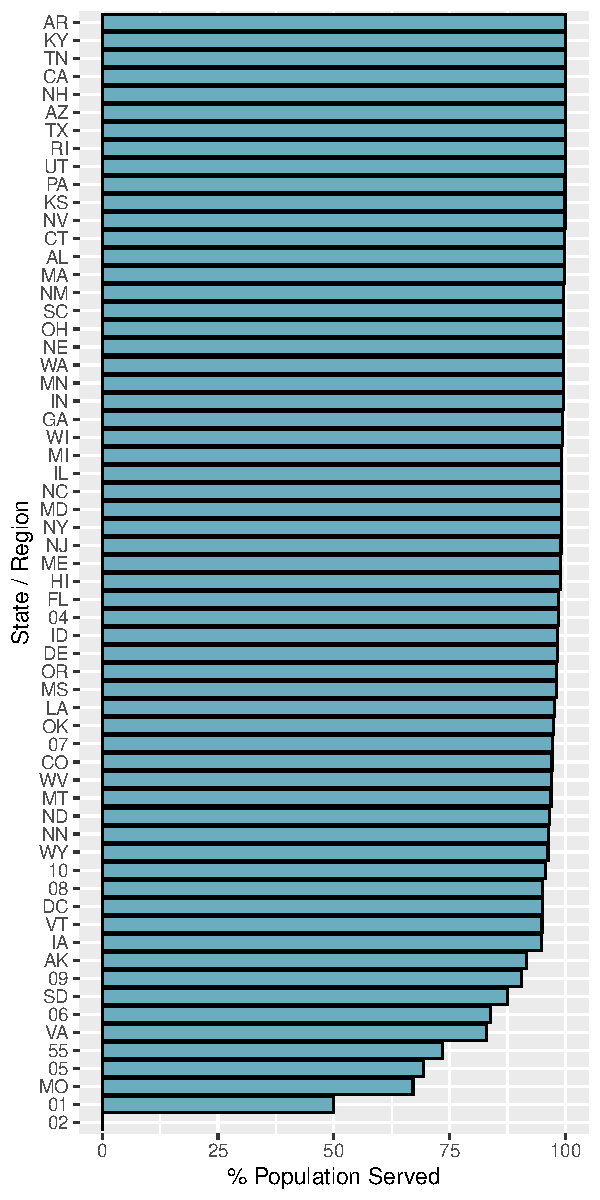
\includegraphics{Documentation_files/figure-pdf/fig-statePopServed-1.pdf}

}

\caption{\label{fig-statePopServed}Bar plot showing the percent of
population served by state or region that is captured by service area
boundaries. Regions refer to tribal systems within that EPA region.}

\end{figure}%

\subsection{Overlapping Boundaries}\label{overlapping-boundaries}

Within the final dataset there are instances where two or more
boundaries occupy the same area. Theoretically two or more systems can
occupy a single block (the spatial scale of the model) but this is known
to be rare. Overlaps usually occur in two scenarios:

\begin{enumerate}
\def\labelenumi{\arabic{enumi}.}
\tightlist
\item
  State boundaries overlapping modeled boundaries:
  Figure~\ref{fig-overlap1} shows an example of Altoona, IA (modeled)
  overlapping the state supplied boundary of Des Moines. In this example
  the modeled boundary for Altoona appears correct. Altoona has a unique
  PWS. However, the state supplied boundary didn't ``erase'' the Altoona
  system from the service area boundary. This conflict is a function of
  course or inaccurate state supplied boundaries.
\end{enumerate}

\begin{figure}

\centering{

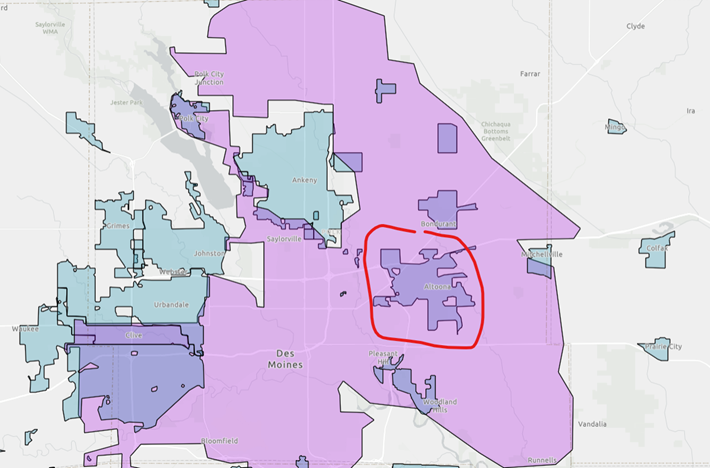
\includegraphics{img/overlap1.png}

}

\caption{\label{fig-overlap1}State boundary (pink) overlapping a modeled
boundary (purple)}

\end{figure}%

\begin{enumerate}
\def\labelenumi{\arabic{enumi}.}
\setcounter{enumi}{1}
\tightlist
\item
  State boundaries overlapping other state boundaries:
  Figure~\ref{fig-overlap2} shows an example of two state systems
  overlapping each other. Because these are state supplied boundaries,
  nothing can be done to resolve this issue. They are either incorrectly
  drawn or multiple systems serve approximately the same areas.
\end{enumerate}

\begin{figure}

\centering{

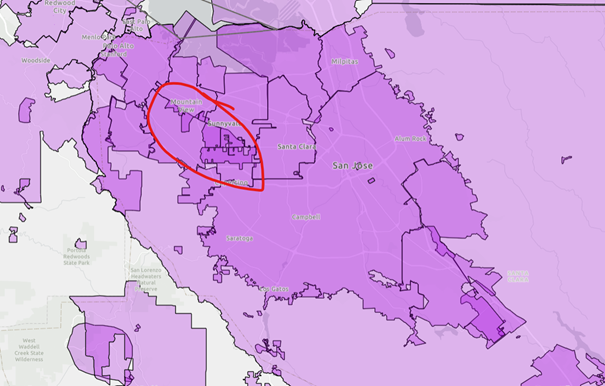
\includegraphics{img/overlap2.png}

}

\caption{\label{fig-overlap2}Multiple California state supplied
boundaries overlapping each other.}

\end{figure}%

\subsection{Incorrect Locations}\label{incorrect-locations}

All models have error. Trying to accurately model such a complex human
phenomenon such as public drinking water infrastructure is difficult.
The drivers that manifest a public drinking infrastructure---economic,
social, environmental---is also complex and varies from state-to-state,
community-to-community. The decision tree model was trained on 3 states
and the random forest was trained on 6 states. This limited geographic
range creates bias in the model and may not represent different drinking
water infrastructure assumptions that may be relevant in one state, but
not in others. One known issue is the poor accuracy of rural water
systems serving very rural geographies. Our decision tree dataset was
trained on states with a fairly urban population and states that didn't
have very many rural water districts to train the model on. South
Dakota, for example, is a state with many rural water districts that
cover large swaths of the rural landscape. We deliberately avoided
including such districts in our training dataset because rural water
districts are unique to only some states. Generally speaking, rural
farmland does not have public water---so we did not want to train a
model that saw farmland as being served by public water. Because of this
model bias, modeled rural water districts are a known issue in our model
and are typically not modeled accurately.

\subsection{Missing Systems}\label{missing-systems}

Why can some systems not be modeled? Besides the issue of systems being
too small to model, there is another reason. The model requires
geographic signals, or clues, to accurately place a service area
boundary on the map. These geographic clues come primarily from two
sources: 1.) SDWIS locations such as wells, intakes, and treatment
plants and 2.) SDWA reported system information such as `City Served'.
These signals help the model triangulate an appropriate geography for
the service area. Approximately a dozen states don't report ``City
Served'. In addition some systems don't have corresponding SDWIS point
locations or the information they provide is incorrect. For these
reasons, a good portion of the systems that could not be modeled were
not modeled. For example, Figure~\ref{fig-missingCon} shows the vast
majority of systems we could not model report less than 100 connections.
Certain types of systems are also difficult to model. As represented in
Figure~\ref{fig-missingType}, the areas we struggle to model are areas
like mobile home park or subdivisions.

\begin{figure}

\centering{

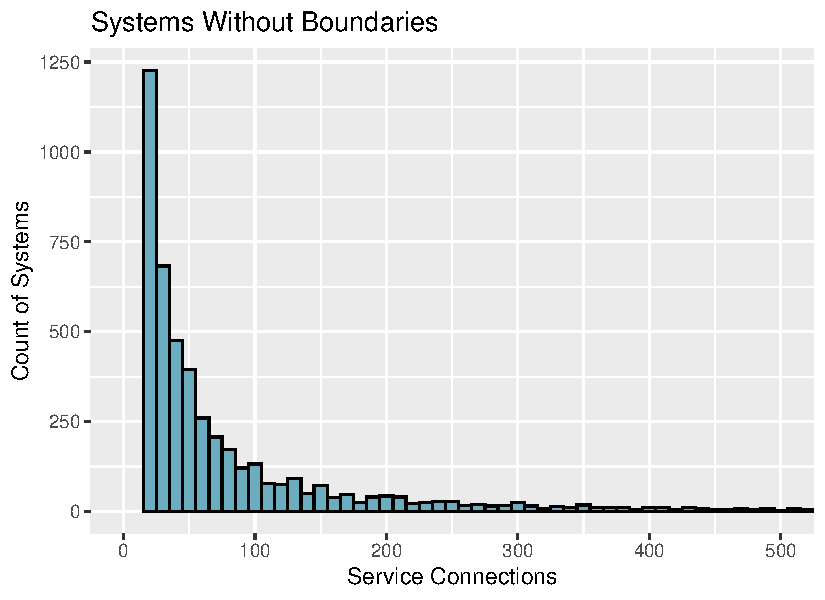
\includegraphics{Documentation_files/figure-pdf/fig-missingCon-1.pdf}

}

\caption{\label{fig-missingCon}Histogram of systems we do not have
boundaries for by the number of service connections reported under SDWA.
binwidth = 10 connections.}

\end{figure}%

\begin{figure}

\centering{

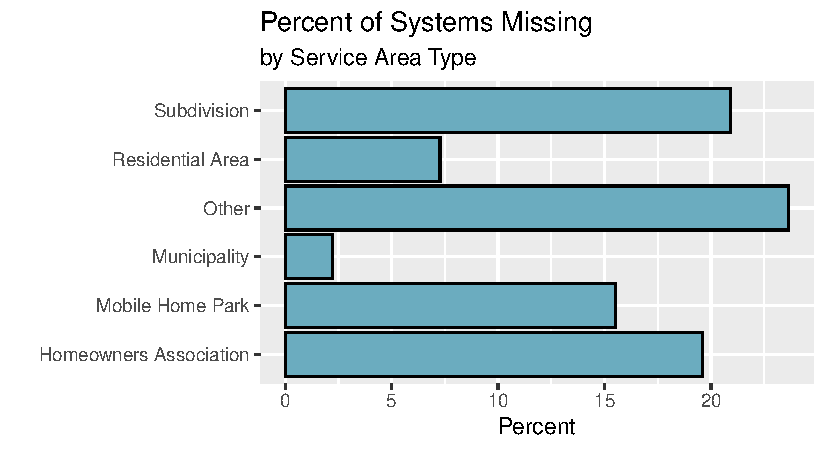
\includegraphics{Documentation_files/figure-pdf/fig-missingType-1.pdf}

}

\caption{\label{fig-missingType}Bar plot showing the percent of systems
missing boundaries by the type of area they primarily serve.}

\end{figure}%

\subsection{Kentucky}\label{kentucky}

You may notice Kentucky's service area boundaries look different from
other state boundaries. In particular, almost the entire area of KY is
covered by public water---and for the most part, Kentucky homes are
almost completely supplied by public water. We received water line data
from the state of kentucky, which delineated the main water lines.
However, we need to delineate the area served by these water lines, not
the two-dimensional line features. To delineate service areas, Voronoi
polygons (also known as Thiessen polygons) were generated from service
line data. It should be noted that the Voronoi polygons were derived
from state supplied data, but the polygons themselves are not state
supplied.

\subsection{Florida}\label{florida}

For some state supplied boundaries in Florida, one polygon was
associated with multiple PWSIDs. We are unable to disaggregate these
multiple systems from their single geography. For these features in the
dataset, you will see multiple PWSIDs within the `PWSID' field.

\phantomsection\label{refs}
\begin{CSLReferences}{1}{0}
\bibitem[\citeproctext]{ref-nngeo}
Dorman, Michael. 2022. \emph{Nngeo: K-Nearest Neighbor Join for Spatial
Data}. \url{https://CRAN.R-project.org/package=nngeo}.

\end{CSLReferences}



\end{document}
